\documentclass[11pt,a4paper]{article}
\usepackage[utf8]{inputenc}
\usepackage[german]{babel}
\usepackage[T1]{fontenc}
\usepackage{amsmath}
\usepackage{amsfonts}
\usepackage{amssymb}
\usepackage{graphicx}
\usepackage[margin=1.25cm]{geometry} % Puts the same margin on all borders of the document

% Packages

\usepackage{hyperref} % Generate hyperlinks to referenced items
\usepackage{adjustbox} % Used to change parameters in \includegraphics[scale=•]{•}
\usepackage{enumitem} % Provides several options for lists
\usepackage{verbatim} % Package to use \begin{comment}
\usepackage{pdfpages} % Used to import PDF pages
\usepackage{multirow} % Allows us to have a single cell in a table span multiple rows
\usepackage{makecell} % Allows us to format multiple lines in a single cell
\usepackage{minted} % Used to syntax highlight code
\usepackage{xcolor}  % Gives access to coloring text
\usepackage{longtable} % Allows us to create a table over multiple pages
\usepackage{float} % Improved placement of floating items
\usepackage{pdfpages} % Used to import pdf pages
\usepackage{booktabs} % Used for horizontal lines instead of \hline



% Settings

\graphicspath{{./files/}} % Sets path for files to the files folder in the same directory

\hypersetup{
    colorlinks=false, %set true if you want colored links
    linktoc=all,     %set to all if you want both sections and subsections linked
    linkcolor=blue,  %choose some color if you want links to stand out
}

\begin{titlepage}
  \title{Algorithmen und Datenstrukturen} % document_name-type_of_document
  \author{Jonas Milkovits}
  \date{Last Edited: \today}
\end{titlepage}

\begin{document}

\pagenumbering{gobble}
\maketitle
\pagenumbering{roman} % i, ii, iii on beginning pages, that don't have content
\tableofcontents
\clearpage
\pagenumbering{arabic} % 1,2,3 on content pages


\section{Einleitung}

\subsection{Probleme in der Informatik}
\begin{itemize}
    \item Problem im Sinne der Informatik
	    \begin{itemize}
          	\item Enthält eine Beschreibung der Eingabe 
          	\item Enthält eine Beschreibung der Ausgabe
          	\item Gibt \textbf{keinen} Übergang von Eingabe und Ausgabe an
          	\item z.B.: Finde den kürzesten Weg zwischen zwei Orten
	    \end{itemize}
	
    \item Probleminstanzen
        \begin{itemize}
          	\item Probleminstanz ist eine konkrete Eingabenbelegung, für die entsprechende Ausgabe gewünscht ist
          	\item z.B.: Was ist der kürzeste Weg vom Audimax in die Mensa?
    	\end{itemize}

\end{itemize}

\subsection{Definitionen für Algorithmen}
\begin{itemize}
    \item Begriff des Algorithmus
        \begin{itemize}
        	\item Endliche Folge von Rechenschritten, der eine Ausgabe in eine Eingabe verwandelt 
        \end{itemize}
        
    \item Anforderungen an Algorithmen
        \begin{itemize}
            \item Spezifizierung der Eingabe und Ausgabe 
              \begin{itemize}
                    \item Anzahl und Typen aller Elemente ist definiert
              \end{itemize}
          \item Eindeutigkeit
              \begin{itemize}
                    \item Jeder Einzelschritt ist klar definiert und ausführbar 
                    \item Die Reihenfolge der Einzelschritte ist festgelegt
              \end{itemize}
            \item Eindlichkeit
              \begin{itemize}
                    \item Notation hat eine endliche Länge
              \end{itemize}
        \end{itemize}

    \item Eigenschaften von Algorithmen
        \begin{itemize}
	    	\item Determiniertheit
	    		\begin{itemize}
	    			\item Für gleiche Eingabe stets die gleiche Ausgabe (andere mögliche Zwischenzustände)
	    		\end{itemize}
	    	\item Determinismus
	    		\begin{itemize}
	    			\item Für gleiche Eingabe stets identische Ausführung und Ausgabe
	    		\end{itemize}
	    	\item Terminierung
	    		\begin{itemize}
	    			\item Algorithmus läuft für jede Eingabe nur endlich lange
	    		\end{itemize}
	    	\item Korrektheit
	    		\begin{itemize}
	    			\item Algorithmus berechnet stets die spezifizierte Ausgabe (falls dieser terminiert)
	    		\end{itemize}
	    	\item Effizienz
	    		\begin{itemize}
	    			\item Sparsamkeit im Ressourcenverbrauch (Zeit, Speicher, Energie,...)
	    		\end{itemize}
	    \end{itemize}
\end{itemize}

\pagebreak

\section{Sortieren}

\subsection{Einführung ins Sortieren}
    \begin{itemize}
        \item \textbf{Das Sortierproblem}
            \begin{itemize}
                \item Ausgangspunkt: Folge von Datensätzen $D_1,D_2,...,D_n$
                \item Zu sortierende Elemente hei\ss en auch Schlüssel(werte)
                \item Ziel: Datensätze so anzuordnen, dass die Schlüsselwerte sukzessive ansteigen/absteigen
                \item Bedingung: Schlüsselwerte müssen vergleichbar sein
                \item Durchführung:
                    \begin{itemize}
                        \item Eingabe: Sequenz von Schlüsselwerten $<a_1,a_2,...,a_n>$
                        \item Engabe ist eine \textbf{Instanz} des Sortierproblems
                        \item Ausgabe: Permutation $<a_1', a_2', ..., a_n'>$ derselben Folge mit Eigenschaft $a_1' \leq ... \leq a_n'$
                    \end{itemize}
                \item Algorithmus \textbf{korrekt}, wenn dieser das Problem für alle Instanzen löst
            \end{itemize}

        \item \textbf{Exkurs: Totale Ordnung}
            \begin{itemize}
                \item Sei $M$ eine nicht leere Menge und $\leq \subseteq MxM$ eine binäre Relation auf $M$
                \item Das Paar $(M, \leq)$ hei\ss t genau dann totale Relation auf der Menge $M$, wenn Folgendes erfüllt ist:
                    \begin{itemize}
                        \item Reflexivität: $\forall x \in M: x \leq x$
                        \item Transitivität: $\forall x,y,z \in M: x \leq y \land y \leq z \Rightarrow x \leq z$
                        \item Antisymmetrie: $\forall x,y \in M: x \leq y \land y \leq x \Rightarrow x = y$
                        \item Totalität: $\forall x,y \in M: x \leq y \lor y \leq x$
                    \end{itemize}
                \item z.B.: $\leq$ Ordnung auf natürlichen Zahlen bildet eine totale Ordnung ($1 \leq 2 \leq 3 ...$)
                \item z.B.: Lexikographische Ordnung $\leq_{lex}$ ist eine totale Ordnung ($A \leq B \leq C ...$)
            \end{itemize}
        
        \item \textbf{Vergleichskriterien von Sortieralgorithmen}
            \begin{itemize}
                \item Berechnungsaufwand $O(n)$
                \item Effizient: Best Case vs Average Case vs Worst Case
                \item Speicherbedarf:
                    \begin{itemize}
                        \item in-place (in situ): Zusätzlicher Speicher von der Eingabegrö\ss e unabhängig
                        \item out-of-place: Speichermehrbedarf von Eingabegrö\ss e abhängig
                    \end{itemize}
                \item Stabilität: Stabile Verfahren verändern die Reihenfolge von äquivalenten Elementen nicht
                \item Anwendung als Auswahlfaktor: 
                    \begin{itemize}
                        \item Hauptoperationen beim Sortieren: Vergleiche und Vertausche
                        \item Diese Operationen können sehr teuer oder sehr günstig sein, je nach Aufwand
                        \item Anpassung des Verfahrens abhängig von dem Aufwand dieser Operationen
                    \end{itemize}    
            \end{itemize}
    \end{itemize}    

    \pagebreak

\subsection{Analyse von Algorithmen - Teil 1} 
    \begin{itemize}

        \item \textbf{Schleifeninvariante (SIV)}
            \begin{itemize}
                \item Sonderform der Invariante 
                \item Am Anfang/Ende jedes Schleifendurchlaufs und vor/nach jedem Schleifendurchlauf gültig
                \item Wird zur Feststellung der Korrektheit von Algorithmen verwendet
                \item Eigenschaften: 
                    \begin{itemize}
                        \item Initialisierung: Invariante ist vor jeder Iteration wahr
                        \item Fortsetzung: Wenn SIV vor der Schleife wahr ist, dann auch bis Beginn der nächsten Iteration
                        \item Terminierung: SIV liefert bei Schleifenabbruch, helfende Eigenschaft für Korrektheit
                    \end{itemize}
                \item Beispiel für Umsetzung: \hyperref[insSortSiv]{\textcolor{red}{Insertion Sort - SIV}}
            \end{itemize}
        
        \item \textbf{Laufzeitanalyse}
            \begin{itemize}
                \item Aufstellung der Kosten und Durchführungsanzahl für jede Zeile des Quelltextes
                \item Beachte: Bei Schleifen wird auch der Aufruf gezählt, der den Abbruch einleitet 
                \item Beispiel für Umsetzung: \hyperref[insSortLaufzeit]{\textcolor{red}{Insertion Sort - Laufzeit}}
                \item Zusätzliche Überprüfung des \texttt{Best Case, Worst Case} und \texttt{Average Case}
            \end{itemize}

        \item \textbf{Effizienz von Algorithmen}
            \begin{itemize}
                \item Effizienzfaktoren
                    \begin{itemize}
                        \item Rechenzeit (Anzahl der Einzelschritte)
                        \item Kommunikationsaufwand 
                        \item Speicherplatzbedarf
                        \item Zugriffe auf Speicher
                    \end{itemize}
                \item Laufzeit hängt von versch. Faktoren ab
                    \begin{itemize}
                        \item Länge der Eingabe
                        \item Implementierung der Basisoperationen
                        \item Takt der CPU 
                    \end{itemize}
            \end{itemize}

    \end{itemize}

\subsection{Analyse von Algorithmen - Teil 2}
    \begin{itemize}
        \item \textbf{Komplexität}
            \begin{itemize}
                \item Abstrakte Rechenzeit $T(n)$ ist abhängig von den Eingabedaten
                \item Übliche Betrachtungsweise der Rechenzeit ist asymptotische Betrachtung
            \end{itemize}
        
        \item \textbf{Asymptotik}
            \begin{itemize}
                \item Annäherung an einer sich ins Unendliche verlaufende Kurve
                \item z.B.: $f(x) = \frac{1}{x} + x$ | Asymptote: $g(x)=x$ | ($\frac{1}{x}$ läuft gegen Null)
            \end{itemize}
        
        \item \textbf{Asymptotische Komplexität}
            \begin{itemize}
                \item Abschätzung des zeitlichen Aufwands eines Algorithmus in Abhängigkeit einer Eingabe
                \item Beispiel für Umsetzung: \hyperref[insSortLaufzeitTheta]{\textcolor{red}{Insertion Sort - Laufzeit $\Theta$}}
            \end{itemize}

        \item \textbf{Asymptotische Notation}
            \begin{itemize}
                \item Betrachtung der Laufzeit $T(n)$ für sehr gro\ss e Eingaben $n \in \mathbb{N}$
                \item Komplexität ist unabhängig von konstanten Faktoren und Summanden
                \item Nicht berücksichtigt: Rechnergeschwindigkeit / Initialisierungsauswände
                \item Komplexitätsmessung via Funktionsklasse ausreichend
                    \begin{itemize}
                        \item Verhalten des Algorithmus für gro\ss e Problemgrö\ss en
                        \item Veränderung der Laufzeit bei Verdopplung der Problemgrö\ss e
                    \end{itemize}
            \end{itemize}
        
        \item \textbf{Gründe für die Nutzung der theoretischen Betrachtung statt der Messung der Laufzeit }
            \begin{itemize}
                \item Vergleichbarkeit
                    \begin{itemize}
                        \item Laufzeit abhängig von konkreter Implementierung und System
                        \item Theoretische Betrachung ist frei von Abhängigkeiten und Seiteneffekten
                        \item Theoretische Betrachtung lässt direkte Vergleichbarkeit zu
                    \end{itemize}
                
                \item Aufwand
                    \begin{itemize}
                        \item Wieviele Testreihen?
                        \item In welcher Umgebung?
                        \item Messen führt in der Ausführung zu hohem, praktischen Aufwand
                    \end{itemize}
                
                \item Komplexitätsfunktion
                    \begin{itemize}
                        \item Wachstumsverhalten ausreichend
                        \item Praktische Evaluation mit Zeiten nur für Auswahl von Systemen mögliche
                        \item Theoretischer Vergleich (Funktionsklassen) hat ähnlichen Erkenntnisgewinn
                    \end{itemize}
            \end{itemize}
    \end{itemize}

\subsection{Analyse von Algorithmen - Teil 3}
    \begin{itemize}
        \item \textbf{$\Theta$-Notation}
            \begin{itemize}
                \item $\Theta$-Notation beschränkt eine Funktion asymptotisch von oben und unten
                \item Funktionen $f,g: \mathbb{N} \rightarrow \mathbb{R}_{>0}$ ($\mathbb{N}$: Eingabelänge, $\mathbb{R}$: Zeit)
                \item[] 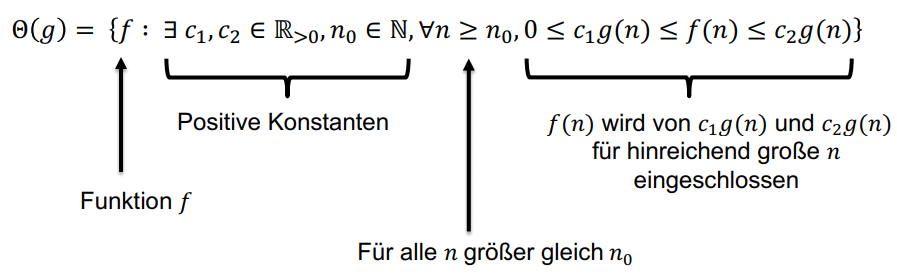
\includegraphics[width=12cm]{thetaNotation.PNG}
                \item $\Theta(g)$ enthält alle $f$, die genauso schnell wachsen wie $g$
                \item Schreibweise: $f \in \Theta(g)$ (korrekt), manchmal auch $f = \Theta(g)$
                \item $g(n)$ ist eine asymptotisch scharfe Schranke von $f(n)$
                \item $f(n)= \Omega(g(n))$ gilt, wenn $f(n) = O(g(n))$ und $f(n)=\Omega(g(n))$ erfüllt sind
                \item[]
                \item[] 
                    \begin{minipage}{0.3\textwidth}
                    \begin{figure}[H]
                        \centering
                        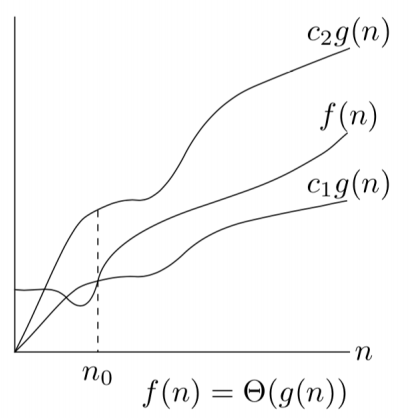
\includegraphics[width=5cm]{thetaNotationGraph.PNG}
                        \caption{Veranschaulichung}
                        \label{}
                    \end{figure}
                    \end{minipage}
                    \begin{minipage}[t]{0.6\textwidth}
                    \vspace{-3cm}
                        \begin{itemize}
                            \item z.B.: $f(n)= \frac{1}{2} n^2 - 3n$ | $f(n) \in \Theta(n^2)$?
                            \item Aus $\Theta(n^2)$ folgt, dass $g(n)=n^2$
                            \item Vorgehen:
                                \begin{itemize}
                                    \item Finden eines $n_0$ und $c_1,c_2$, sodass
                                    \item $c_1*g(n) \leq f(n) \leq c_2*g(n)$ erfüllt ist
                                    \item Konkret: $c_1*n^2 \leq \frac{1}{2} n^2 - 3n \leq c_2*n^2$
                                    \item Division durch $n^2$: $c_1 \leq \frac{1}{2}-\frac{3}{n} \leq c2$
                                    \item Ab $n=7$ positives Ergebnis: $0,0714$ | $n_0 = 7$
                                    \item Deswegen setzen wir $c_1=\frac{1}{14}$
                                    \item Für $n \rightarrow \infty: ~ 0,5$ | $c_2 = 0,5$
                                    \item Natürlich auch andere Konstanten möglich
                                \end{itemize}
                        \end{itemize}
                    \end{minipage}
            \end{itemize}

        \item \textbf{$O$-Notation}
            \begin{itemize}
                \item $O$-Notation beschränkt eine Funktion asymptotisch von oben
                \item[] 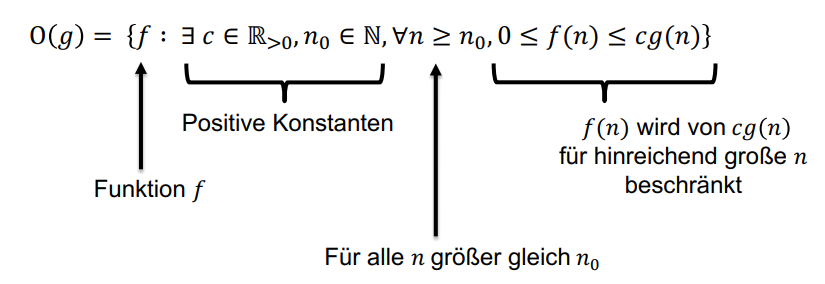
\includegraphics[width=12cm]{oNotation.PNG}
                \item $O(g)$ enthält alle $f$, die höchstens so schnell wie $g$ wachsen
                \item Schreibweise: $f=O(g)$
                \item $f(n)=\Theta(g) \rightarrow f(n) = O(g)$ | $\Theta(g(n)) \subseteq O(g(n))$
                \item Ist $f$ in der Menge $\Theta(g)$, dann auch in der Menge $O(g)$
                \item[]
                \item[] 
                    \begin{minipage}{0.3\textwidth}
                    \begin{figure}[H]
                        \centering
                        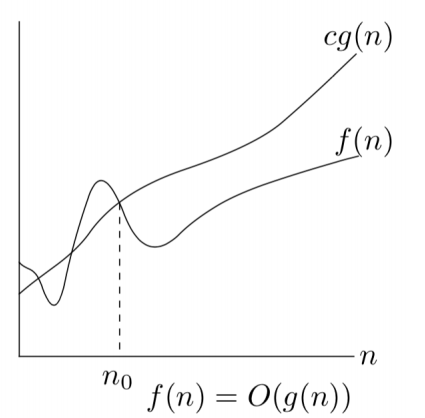
\includegraphics[width=5cm]{oNotationGraph.PNG}
                        \caption{Veranschaulichung}
                        \label{}
                    \end{figure}
                    \end{minipage}
                    \begin{minipage}[t]{0.6\textwidth}
                    \vspace{-3cm}
                        \begin{itemize}
                            \item z.B.: $f(n) = n + 2$ | $f(n) = O(n)$?
                            \item Ja $f(n)$ ist Teil von $O(n)$ für z.B. $c = 2$ und $n_0 = 2$
                        \end{itemize}
                    \end{minipage}
            \end{itemize}
        
        \item \textbf{$O$-Notation Rechenregeln}
            \begin{itemize}
                \item Konstanten: 
                    \begin{itemize}
                        \item $f(n) = a$ mit $a \in \mathbb{R}$ konstante Funktion $\rightarrow$ $f(n) = O(1)$
                        \item z.B. $3 \in O(1)$
                    \end{itemize}
                
                \item Skalare Multiplikation:
                    \begin{itemize}
                        \item $f= O(g)$ und $a \in \mathbb{R}$ $\rightarrow$ $a*f = O(g)$
                    \end{itemize}
                
                \item Addition: 
                    \begin{itemize}
                        \item $f_1 = O(g_1)$ und $f_2 = O(g_2)$ $\rightarrow$ $f_1+f_2= O(max\{g_1,g_2\})$
                    \end{itemize}
                
                \item Multiplikation:
                    \begin{itemize}
                        \item $f_1 = O(g_1)$ und $f_1 = O(g_2)$ $\rightarrow$ $f_1*f_2= O(g_1*g_2)$
                    \end{itemize}
            \end{itemize}
        
        \item \textbf{$\Omega$-Notation}
            \begin{itemize}
                \item $\Omega$-Notation beschränkt eine Funktion asymptotisch von unten
                \item[] 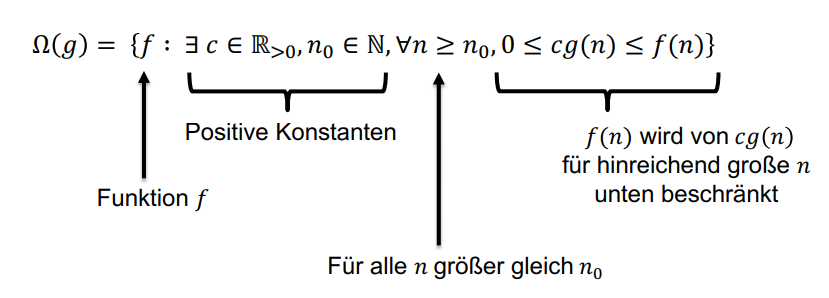
\includegraphics[width=12cm]{omegaNotation.PNG}
                \item $\Omega$-Notation enthält alle $f$, die mindestens so schnell wie $g$ wachsen
                \item Schreibweise: $f = \Omega(g)$
                \item[]
                \item[] 
                    \begin{minipage}{0.3\textwidth}
                    \begin{figure}[H]
                        \centering
                        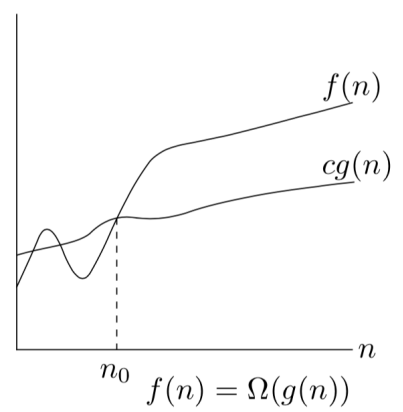
\includegraphics[width=5cm]{omegaNotationGraph.PNG}
                        \caption{Veranschaulichung}
                        \label{}
                    \end{figure}
                    \end{minipage}
                    \begin{minipage}[t]{0.6\textwidth}
                    \vspace{-3cm}
                    \end{minipage}
            \end{itemize}
        
        \item \textbf{Komplexitätsklassen}
            \begin{itemize}
                \item $n$ ist hier die Länge der Eingabe
                \item[] \includegraphics[width=12cm]{komplexitätsklassen.PNG}
                \item Ausführungsdauer, falls eine Operation $n$ genau $1\mu s$ dauert 
                \item[] \includegraphics[width=12cm]{komplexitätsklassenDauer.PNG}
            \end{itemize}
        
        \item Asymptotische Notationen in Gleichungen
            \begin{itemize}
                \item $2n^2 + 3n + 1 = 2n^2 + \Theta(n)$
                \item $\Theta(n)$ fungiert hier als Platzhalter für eine beliebige Funktion $f(n)$ aus $\Theta(n)$
                \item z.B.: $f(n) = 3n + 1$
            \end{itemize}
        
        \item \textbf{$o$-Notation}
            \begin{itemize}
                \item $\o$-Notation stellt eine echte obere Schranke dar
                \item Ausschlaggebend ist, dass es für alle $c \in \mathbb{R}_{>0}$ gelten muss
                \item Au\ss erdem $<$ statt $\leq$
                \item z.B.: $2n = o(n^2)$ und $2n^2 \neq o(n^2)$ 
                \item[] 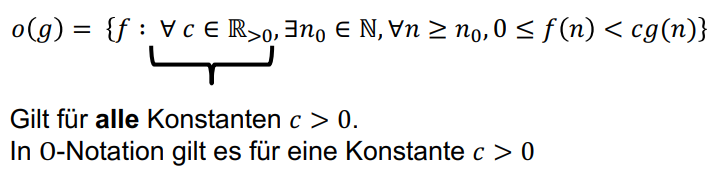
\includegraphics[width=12cm]{oKleinNotation.PNG}
                
            \end{itemize}
        
        \item \textbf{$\omega$-Notation}
            \begin{itemize}
                \item $\omega$-Notation stellt eine echte untere Schranke dar
                \item Ausschlaggebend ist, dass es für alle $c \in \mathbb{R}{>0}$ gelten muss
                \item Au\ss erdem $>$ statt $\geq$
                \item z.B.: $\frac{n^2}{2} = \omega(n)$ und $\frac{n^2}{2} \neq \omega(n^2)$
                \item[] 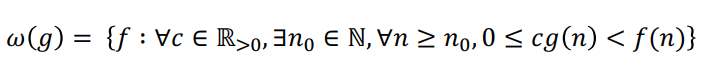
\includegraphics[width=12cm]{omegaKleinNotation.PNG}
            \end{itemize}
    \end{itemize}

\subsection{Insertion Sort}
    \begin{itemize}
        \item \textbf{Idee}
            \begin{itemize}
                \item Halte die linke Teilfolge sortiert
                \item Füge nächsten Schlüsselwert hinzu, indem es an die korrekte Position eingefügt wird
                \item Wiederhole den Vorgang bis Teilfolge aus der gesamten Liste besteht
            \end{itemize}
        
        \item \textbf{Code}
            \begin{minted}[gobble = 9]{c}  
            FOR j = 1 TO A.length - 1
              key = A[j]
              // Füge A[j] in die sortierte Sequenz A[0...j-1] ein
              i = j - 1
              WHILE i >= 0 and A[i] > key
                  A[i + 1] = A[i]
                  i = i - 1
              A[i + 1] = key
            \end{minted}
        \item \textbf{Schleifeninvariante von \texttt{Insertion Sort}} {\label{insSortSiv}} 
            \begin{itemize}
                \item Zu Beginn jeder Iteration der \texttt{for}-Schleife besteht die Teilfolge \texttt{A[0...j-1]} aus den Elementen \\
                der ursprünglichen Teilfolge \texttt{A[0...j-1]} enthaltenen Elementen, allerdings in sortierter Reihenfolge.
            \end{itemize}

        \item \textbf{Korrektheit von \texttt{Insertion Sort}}
            \begin{itemize}
                \item Initialisierung:
                    \begin{itemize}
                        \item   Beginn mit \texttt{j=1}, also Teilfeld \texttt{A[0...j-1]} besteht nur aus einem Element \texttt{A[0]}. \\
                                Dies ist auch das ursprüngliche Element und Teilfeld ist sortiert.
                    \end{itemize}

                \item Fortsetzung:
                    \begin{itemize}
                        \item   Zu zeigen ist, dass die Invariante bei jeder Iteration erhalten bleibt. Ausführungsblock der \texttt{for}-Schleife
                                sorgt dafür, dass \texttt{A[j-1], A[j-2]},... je um Stelle nach rechts geschoben werden bis \texttt{A[j]} korrekt eingefügt wurde. 
                                Teilfeld \texttt{A[0...j]} besteht aus ursprünglichen Elementen und ist sortiert. Inkrementieren von j erhält die Invariante.
                    \end{itemize}

                \item Terminierung: 
                    \begin{itemize}
                        \item   Abbruchbedingung der \texttt{for}-Schleife, wenn \texttt{j > A.length - 1}. Jede Iteration erhöht j.
                                Dann bei Abbruch ist \texttt{j = n } und einsetzen in Invariante liefert das Teilfeld \texttt{A[0...n-1]}
                                welches aus den ursprünglichen Elementen besteht und sortiert ist. Teilfeld ist gesamtes Feld.
                    \end{itemize}

                \item Algorithmus \texttt{Insertion Sort} arbeitet damit korrekt.
                
            \end{itemize}
        
        \item \textbf{Laufzeitanalyse von \texttt{Insertion Sort}} {\label{insSortLaufzeit}}
            \begin{itemize}
                \item[] 
                    \begin{minipage}{0.45\textwidth}
                    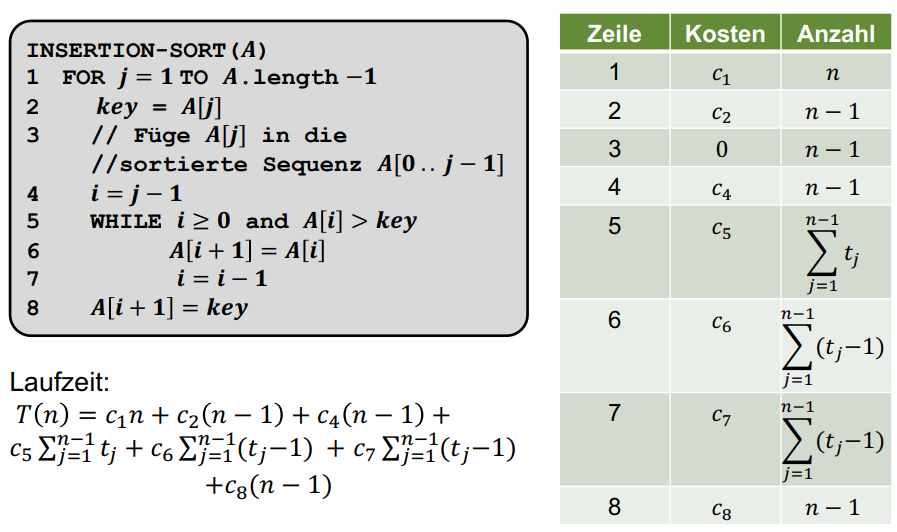
\includegraphics[width=8cm]{insSortLaufzeit.PNG}
                    \end{minipage}
                    \begin{minipage}[t]{0.45\textwidth}
                    \vspace{-2.5cm}
                    \begin{itemize}
                        \item Festlegung der Laufzeit für jede Zeile
                        \item Jede Zeile besitzt gewissen Kosten \texttt{$c_i$}
                        \item Jede Zeile wird $x$ mal durchgeführt 
                        \item $Laufzeit = Anzahl * Kosten$ jeder Zeile
                        \item Schleifen: Abbruchüberprüfung zählt auch
                        \item \texttt{$t_j$}: Anzahl der Abfragen der \texttt{While}-Schleife
                    \end{itemize}
                    \end{minipage}

                \item Warum $n$ in Zeile 1?
                    \begin{itemize}
                        \item Die Überprüfung der Fortführungsbedingung beinhaltet auch die letze Überprüfung 
                        \item Quasi die Überprüfung, durch die die Schleife abbricht
                    \end{itemize}

                \item Warum $\sum^{n-1}_{j=1}$ in Zeile 5?
                    \begin{itemize}
                        \item Aufsummierung aller einzelnen $t_j$ über die Anzahl der Schleifendurchläufe
                        \item Diese ist allerdings $n-1$ und nicht $n$, da die Abbruchüberprüfung dort auch enthalten ist
                    \end{itemize}
                
                \item Warum $t_j-1$ in Zeile 6?
                    \begin{itemize}
                        \item Selbes Argument wie oben, bei $t_j$ ist die Abbruchüberprüfung enthalten
                        \item Deswegen wird die \texttt{while}-Schleife nur $t_j-1$-mal ausgeführt
                    \end{itemize}
                
                \item \texttt{Best Case}
                    \begin{itemize}
                        \item zu sortierendes Feld ist bereits sortiert 
                        \item $t_j$ wird dadurch zu 1, da die \texttt{While}-Schleife immer nur einmal prüft (Abbruch)
                        \item Die zwei Zeilen innerhalb der \texttt{While}-Schleife werden nie ausgeführt
                        \item Durch Umformen ergibt sich, dass die Laufzeit eine lineare Funktion in $n$ ist
                    \end{itemize}
                
                \item \texttt{Worst Case}
                    \begin{itemize}
                        \item zu sortierendes Feld ist umgekehrt sortiert 
                        \item $t_j$ wird dadurch zu $j+1$, da die \texttt{While}-Schleife immer die gesamte Länge prüft
                        \item Durch Umformen ergibt sich, dass die Laufzeit eine quadratische Funktion in $n$ ist ($n^2$)
                    \end{itemize}
                
                \item \texttt{Average Case} 
                    \begin{itemize}
                        \item im Mittel gut gemischt 
                        \item $t_j$ wird dadurch zu $j/2$
                        \item Die Laufzeit bleibt aber eine quadratische Funktion in $n$ ($n^2$)
                    \end{itemize}
            \end{itemize}
        
        \item \textbf{Asymptotische Laufzeitbetrachtung $\Theta$} {\label{insSortLaufzeitTheta}}
            \begin{itemize}
                \item $T(n)$ lässt sich als quadratische Funktion $an^2 + bn + c$ betrachten 
                \item Terme niedriger Ordnung sind für gro\ss e $n$ irrelevant
                \item Deswegen Vereinfachung zu $n^2$ und damit $\Theta(n^2)$
            \end{itemize}
    \end{itemize}
    
\subsection{Bubble Sort}

    \begin{itemize}
        \item \textbf{Idee}
            \begin{itemize}
                \item Vergleiche Paare von benachbarten Schlüsselwerten
                \item Tausche das Paar, falls rechter Schlüsselwert kleiner als linker
            \end{itemize}
        
        \item \textbf{Code}
            \begin{minted}[gobble = 9]{c}  
            FOR i = 0 TO A.length - 2
                FOR j = A.length - 1 DOWNTO i + 1
                    IF A[j] < A[j-1]
                        SWAP(A[j], A[j-1])
            \end{minted}

        \item \textbf{Analyse von \texttt{Bubble Sort}}
            \begin{itemize}
                \item Anzahl der Vergleiche:
                    \begin{itemize}
                        \item Es werden stets alle Elemente der Teilfolge miteinander verglichen
                        \item Unabhängig von der Vorsortierung sind \texttt{Worst} und \texttt{Best Case} identisch
                    \end{itemize}
                
                \item Anzahl der Vertauschungen:
                    \begin{itemize}
                        \item \texttt{Best Case}: 0 Vertauschungen
                        \item \texttt{Worst Case}: $\frac{n^2-n}{2}$ Vertauschungen
                    \end{itemize}
                
                \item Komplexität:
                    \begin{itemize}
                        \item \texttt{Best Case}: $\Theta(n)$
                        \item \texttt{Average Case}: $\Theta(n^2)$
                        \item \texttt{Worst Case}: $\Theta(n^2)$
                    \end{itemize}
            \end{itemize}
        
    \end{itemize}

\pagebreak

\section{Pseudocode in der Vorlesung AuD}

\begin{itemize}
    \item Datentypen
        \begin{itemize}
	    	\item String
	    		\begin{itemize}
	    			\item Aufbau: \mint{c}|"Die Summe ist"|
	    			\item Konkatenation: \mint{c}|"Die Summe ist" summe|  
                \end{itemize}
            \item Array
                \begin{itemize}
                    \item \texttt{A}: Bezeichung eines Arrays \texttt{A}
                    \item \texttt{A[i]} Zugriff auf \texttt{(i+1)}-tes Element des Arrays
                \end{itemize}
        \end{itemize}

    \item Methoden
        \begin{itemize}
            \item Rückgabe:
                \mint{c}|return summe| 
        \end{itemize}

    \item Schleifen 
        \begin{itemize}
	    	\item While-Schleife 
            \item[]
                \begin{minted}[autogobble]{c}  
                    WHILE summe <= n // Falls j = 1 to A.length -1: to ist dasselbe wie <=
                        summe = summe + 1
                    ENDWHILE
                \end{minted}
        \end{itemize}
    
    \item Variablen
        \begin{itemize}
            \item Initialisierung
            \item[] \mint{c}|summe := 0| 
        \end{itemize}

\end{itemize}



\end{document}